\chapter{Learning speech act categories}
\label{chap:eng-sp}


Learners of both (perhaps all) languages face a further difficulty. Besides their main function of eliciting information, interrogative clauses can also be used to fulfill a range of other conventional functions. Test questions like (\ref{bg-prag:test}) do not present the asker as lacking information; parents can use questions like (\ref{bg-prag:ped}) to teach children object labels; indirect requests like (\ref{bg-prag:req}) are not genuinely soliciting information; and rhetorical questions act similar to assertions (\ref{bg-prag:rhe}). Such uses of interrogatives might mask the association of interrogatives with information-seeking speech acts. Additionally, other clause types like declaratives can be used as questions (e.g. rising declaratives, \citealt{gunlogson2004,gunlogson2008,jeong2018,rudin2018}). All these are potential sources of noise in the input with respect to the mapping between form and function.

\bex{bg-prag:types}
\bxl\label{bg-prag:test}
What is H$_{2}$O?		\hfill \tit{Test}
\ex \label{bg-prag:ped}
What's this?	\hfill \tit{Pedagogy}
\exl
\eex

\bex{}
\bxl\label{bg-prag:req}
Can you pass the salt?			\hfill \tit{Request}
\ex \label{bg-prag:rhe}
Are you crazy?	\hfill \tit{Rhetorical}
\exl
\eex


Common to all the functions listed above is the fact that in a conversation, questions expect responses (\citealt{duncan1972turn}). In turn-taking theory, questions usually mark the turn-transition points: after a question, the current speaker yields their turn and appoint the next speaker while the other participants of the conversation would pick up the turn by answering the question (\citealt{kendon1967gaze, argyle1972gaze, levinson1983, tice2011turn} among others, see \citealt{enfield2010} for a survey).  Additionally, questions are argued to set up the topics and issues in a conversation (\citealt{roberts2012,farkasbruce2010}), and speakers could use questions to keep track of where they are in a conversation. Therefore, despite the fact that questions can be used to fulfill many functions, the role of questions in a conversation seems to be clear: speakers use questions to solicit responses and set up topics for discussion. If children are sensitive to signals of response expectations or topic settings, they could make use of that information to identify questions, and, in turn, interrogatives. 
%As mentioned above, combining syntactic and prosodic information may explain some mismatches, as with the case of rising declaratives. Other syntactic markers might be helpful as well: many have noted that interrogatives that function like imperatives tend to take specific forms such as having modals like (\ref{bg-prag:req}), or \tit{why don't} and \tit{why not} interrogatives (i.e. \tit{whimperatives}, \citealt{sadock1974, green1975whimp}).


we will annotate the social function of each utterance. Our preliminary results in Fig.~\ref{fig:uttgoals} show that this prediction is borne out: parents tend to use questions to direct infants’ attention to new objects in their surrounding, while assertions are used to teach and express opinions.

\begin{table}[H]
\begin{center}
\begin{tabular}{c|p{6cm}|c}
\hline
Social Function&Explanation	&\tit{Example}\\
\hline
\hline
Attention& Direct attention to new object&\tit{Alex, Look!}\\
\hline
Negotiating & Negotiating about carrying out an action	&\tit{You read it to mommy.}\\
\hline
Teaching& Teaching the child about something or how to do things &\tit{What’s that (pointing to a bumblebee)?}\\
\hline
Discussing & Exchanging information but not for pedagogical purposes &\tit{Do you like scratchy cat kisses?}\\
\hline
Verbal Routines& Routines in social situations/games &\tit{Ready? Go!}\\
\hline
Emoting& Expressing emotions like excitement &\tit{Yay!}\\
\hline
Imitating & Imitating sounds, repeating others' utterances &\tit{vroom vroom!}\\
\hline
Meta-communication & Seeking clarification, confirmation, acknowledgement of another utterance/action	&\tit{ (after Alex makes some noise) What?}\\
\hline
\end{tabular}
\end{center}
\label{code:social}
\vspace{-4ex}
\caption{ Types of social functions of parents’ utterances}
\end{table}



%\vspace{-3ex}
%\noindent 
The other property of interest is that they expect responses. For conversations with pre-linguistic infants, this may mean that parents wait longer after questions for a response. Thus, in this project, we plan to measure the length of pause between parents’ consecutive utterances like (\ref{code-prag:pause}). To do so, we will first extract the consecutive turn sequences in parents’ speech. Following \cite{reimchen2017}, we define such sequences as a sequence of utterances spoken by the same speaker on the same topic. Within the sequences, we will measure the length of pauses between utterances, and see if parents pause longer after questions than after assertions. Moreover, we will code whether a question in the sequence is followed by another question, since \cite{reimchen2017} observe that parents to 14-month-olds tend to follow questions with another question. Our preliminary results show that parents are equally likely to ask another question as they are to answer their own questions, but parents tend to pause longer after questions (mean $= 1861ms$, Fig.~\ref{fg:pauses}) than assertions (mean $= 1216ms; t(347) = 2.08, p <0.05$): parents wait for responses after asking a question but proceed with the conversation after an assertion. 




\bex{code-prag:pause}
%\bxl{}
\tbf{Consecutive turn sequence}\\ 
%Alex's mother: Who’s that? [pause: 1.086s] Is that the postman?	\hfill		
\bxl
\ex You can’t take your rake on the swing but you can [pause: 0.014s] You wanna take your big bird rake on the swing? 			\hfill \tsc{Assertion -Question}
\ex You don't wanna swing? [pause: 0.23s]	You don’t have to.	\hfill \tsc{Question-Assertion}
\ex Here you use this one. [pause: 0.033s] This one works better.	\hfill \tsc{Assertion-Assertion}
\exl
\eex


%\begin{figure}[H]
%\begin{center}
%	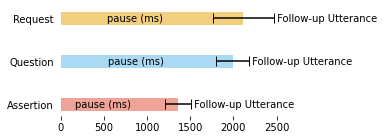
\includegraphics[width = 0.5\textwidth]{q-followup.png}
%	\caption{Duration of pause (ms) after each speech act}\label{fg:pauses}
%\end{center}
%\end{figure}


Another consequence of the response-expectation property of questions is that by the end of a question, the speaker tends to appoint the next speaker. A common device for turn allocation is eye gaze (\citealt{argyle1972gaze, kendon1967gaze,duncan1979gaze, rossano2009gaze}), so the \hypos{} predicts that parents would engage in longer eye contact after questions than other types of speech acts. To test this, we plan to annotate, on a second-by-second basis, parents' attentional behaviors toward the child using ELAN. The annotation will be done without reference to the transcript so that the annotator is not biased by the linguistic information of the scene. For each video, the annotators will first identify the segments of the video where the parent and the child are both visible on screen, and the parent’s focus of attention is identifiable via her visual focus or head/body orientation. Then for these segments, we will annotate whether the parent is attending to the child.  


\begin{figure}[H]
\label{fg:attention}
\begin{center}
	%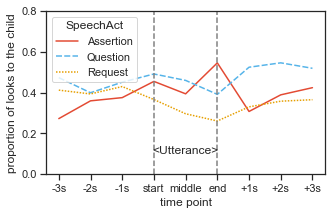
\includegraphics[width =0.4\textwidth]{q-attention.png}
	\vspace{-6ex}
	\caption{Proportion of parents' looks to the child (preliminary results)}
\end{center}
\end{figure}


Fig.~\ref{fg:attention} shows the proportion of looks to the child before and after uttering a sentence in our pilot sample: when the utterance is a question, the proportion of looks to the child is higher ($0.47$) than when it is an assertion ($0.39; t(16) = 2.53, p <0.05$) or a request ($0.35; t(16)= 4.55, p<0.001$); in the post-utterance region, the proportion of looks to the child is higher when the utterance is a question ($0.53$) than when it is an assertion ($0.37; t(4) = 4.4, p<0.05$) or a request ($0.35; t(4) = 13.2, p<0.001$). These results suggest that the predictions of the \hypos{} are borne out: parents look at the child longer after questions. Thus, despite parents asking questions whose answers they know, the characteristic turn-changing properties of questions are observable in speech pauses and speaker attention. 



\subsubsection{Syntactic features}\label{prop-code:syn}
 \noindent\emph{For Study~1 (English)}:
We expect most interrogatives to have subject-auxiliary inversion, although there might be many exceptions. Thus, we plan to annotate the relative positions of the subject and auxiliary to empirically test this prediction. Our pilot results suggest that inversion is indeed the dominant pattern, with 92\% of the interrogative clauses having auxiliaries preceding the subject. 